\documentclass[12pt]{../../oss-apphys-exam}
\usepackage{enumitem}

\tikzstyle{every node}=[scale=.8]

\runningheader{
  \fontfamily{phv}\small
  \textcolor{gray}{AP PHYSICS C: ELECTRICITY AND MAGNETISM $\blacksquare$}
  \textbf{MULTIPLE-CHOICE QUESTIONS}}{}{}


\begin{document}

\begin{center}
  {
    \fontfamily{phv}\Large
    \textbf{PHYSICS C: ELECTRICITY AND MAGNETISM\\
      SECTION I\\
      TIME -- 30 MINUTES}
  }
\end{center}

\textbf{Directions:} Each of the questions or incomplete statements below is
followed by five suggested answers or completions. Select the one that is best
in each case and place the letter of your choice in the corresponding box on
the student answer sheet.

\begin{questions}
  \question Three long, current-carrying wires are shown in the cross-sectional
  view below. The currents in wires R and S are out of the page, and the
  current in wire T is into the page. The currents in the wires have equal
  magnitude, and the wires are in the positions shown. Point P is halfway
  between wires S and T. If $B_S$ is the magnitude of the magnetic field at
  point P due to wire S, which of the following gives the magnitude and
  direction of the magnetic field at point P due to all three wires?
  \uplevel{
    \centering
    \begin{tikzpicture}[scale=.8]
      \draw[axes] (0,0)--(10,0) node[right]{$x$};
      \draw[very thick,fill=white] (2,0) circle (.3) node[below=7]{Wire R};
      \fill (2,0) circle (.2);
      \draw (2,.3)--(2,.7) node[above]{$x=0$};

      \draw[very thick,fill=white] (4,0) circle (.3) node[below=7]{Wire S};
      \fill (4,0) circle (.2);
      \draw (4,.3)--(4,.7) node[above]{$x=d$};
      
      \fill (6,0) circle (.1) node[below right]{P};

      \draw[very thick,fill=white] (8,0) circle (.3) node[below=7]{Wire T};
      \begin{scope}[ultra thick,rotate around={45:(8,0)}]
        \draw (7.7,0)--(8.3,0);
        \draw (8,.3)--(8,-.3);
      \end{scope}
      \draw (8,.3)--(8,.7) node[above]{$x=3d$};
    \end{tikzpicture}
  }
  
  \begin{tabular}{lll}
    & \textbf{Magnitude} & \textbf{Direction}\\
    \hline
    (A) & $B_S/2$  & Top of the page \\
    (B) & $B_S/2$  & Bottom of the page \\
    (C) & $B_S$    & Top of the page \\
    (D) & $5B_S/2$ & Top of the page \\
    (E) & $5B_S/2$ & Bottom of the page
  \end{tabular}

  \question Two wires perpendicular to the $x$-axis have currents $I$ directed
  out of the page, as shown below. Each wire is a distance $d$ from the
  $y$-axis. Point P lies on the $y$-axis at the coordinate $(0,a)$, and point R
  lies on the x-axis at the coordinate $(-d/2,0)$. Which of the following
  expressions represents the magnitude of the magnetic field at point R?
  \uplevel{
    \centering
    \begin{tikzpicture}[scale=.75]
      \draw[axes] (-4,0)--(4,0) node[right]{$x$};
      \draw[axes] (0,-1)--(0,3.5) node[above]{$y$};
      \draw[very thick,fill=white] (-3,0) circle (.3) node[above left=4]{$I$};
      \fill (-3,0) circle (.15);

      \draw[very thick,fill=white] (3,0) circle (.3) node[above right=4]{$I$};
      \fill (3,0) circle (.15);

      \fill (0,2.5) circle (.08) node[left]{P};
      \fill (-1.5,0) circle (.08) node[above left]{R};
      
      \begin{scope}[<->|]
        \draw (.3,0)--+(0,2.5) node[midway,fill=white]{$a$};
        \draw (0,-.5)--+(3,0) node[midway,fill=white]{$d$} node[below]{Wire 2};
        \draw (0,-.5)--+(-3,0) node[midway,fill=white]{$d$} node[below]{Wire 1};
        \draw (0,.3)--+(-1.5,0) node[midway,above]{$d/2$};
      \end{scope}
    \end{tikzpicture}
  }
  \begin{choices}
    \choice Zero
    \choice $\dfrac{\mu_oI}{2\pi d}$
    \choice $\dfrac{\mu_oI}{\pi d}$
    \choice $\dfrac{4\mu_oI}{3\pi d}$
    \choice $\dfrac{2\mu_oI}{3\pi d}$
  \end{choices}
  \newpage

  \uplevel{
    \centering
    \begin{tikzpicture}[thick]
      \draw (1.75,.35)--(1.2,0) node[midway,above left]{$S$}--(0,0)
      to[battery1,l=$\mathcal E$] (0,2) to[R,l=$R$] (4,2) to[C,l=$C$]
      (4,0)--(1.8,0);
    \end{tikzpicture}
  }
  \question The capacitor $C$ in the circuit shown above is initially
  uncharged. The switch $S$ is then closed. Which of the following best
  represents the voltage $V_R$ across the resistor $R$ as a function of time
  $t$?
  
  \begin{oneparchoices}
    \choice
    \hspace{-.2in}
    \begin{tikzpicture}
      \draw[axes] (0,0)--(2,0) node[right]{$t$};
      \draw[axes] (0,0)--(0,2) node[right]{$V_R$};
      \draw[very thick] (0,0)--(1.8,1.6);
      \draw (.1,1.6)--(-.1,1.6) node[left]{$\mathcal E$};
    \end{tikzpicture}

    \choice
    \hspace{-.2in}
    \begin{tikzpicture}
      \draw[axes] (0,0)--(2,0) node[right]{$t$};
      \draw[axes] (0,0)--(0,2) node[right]{$V_R$};
      \draw[very thick] (0,1.6)--(1.8,0);
      \draw (.1,1.6)--(-.1,1.6) node[left]{$\mathcal E$};
    \end{tikzpicture}

    \choice
    \hspace{-.2in}
    \begin{tikzpicture}
      \draw[axes] (0,0)--(2,0) node[right]{$t$};
      \draw[axes] (0,0)--(0,2) node[right]{$V_R$};
      \draw (.1,1.6)--(-.1,1.6) node[left]{$\mathcal E$};
      \draw[very thick,domain=0:1.6] plot(\x,{1.6*(1-exp(-3*\x))});
    \end{tikzpicture}

    \choice
    \hspace{-.2in}
    \begin{tikzpicture}
      \draw[axes] (0,0)--(2,0) node[right]{$t$};
      \draw[axes] (0,0)--(0,2) node[right]{$V_R$};
      \draw (.1,1.6)--(-.1,1.6) node[left]{$\mathcal E$};
      \draw[very thick,domain=0:1.6] plot(\x,{1.6*exp(-3*\x))});
    \end{tikzpicture}

    \choice
    \hspace{-.2in}
    \begin{tikzpicture}
      \draw[axes] (0,0)--(2,0) node[right]{$t$};
      \draw[axes] (0,0)--(0,2) node[right]{$V_R$};
      \draw (.1,1.6)--(-.1,1.6) node[left]{$\mathcal E$};
      \draw[very thick,domain=0:1.7] plot(\x,{1.6*(1-exp(3.5*(\x-1.7)))});
    \end{tikzpicture}
  \end{oneparchoices}

  \uplevel{
    \textbf{Question \ref{rcirc1}--\ref{rcirc2}}
    \begin{center}
      \begin{tikzpicture}[thick,scale=1.4]
        \draw (0,0) to[battery1,l=\SI{12}\volt] (0,2)--(1.25,2)
        to[R,l=\SI2\ohm] (2.5,2) to[R,l=\SI2\ohm] (3.75,2)--(4,2)--(4,0)--(0,0);
        \draw (1.25,2)--(1.25,1) to[R,l=\SI2\ohm] (3.75,1)--(3.75,2);
        \fill (1.25,2) circle (.05) node[above]{A};
        \fill (2.5,2) circle (.05) node[above]{B};
        \fill (3.75,2) circle (.05) node[above]{C};
        \draw[fill=white] (.4,1.85) rectangle (.9,2.15) node[midway]{Fuse};
      \end{tikzpicture}
    \end{center}
    An electric circuit consists of a \SI{12}{\volt} battery, an
    ideal \SI{10}{\ampere} fuse, and three \SI2{\ohm} resistors connected as
    shown above.
    }
  \question What would be the reading on a voltmeter connected across points A
  and C?
  \label{rcirc1}
  \begin{choices}
    \choice\SI{12}\volt
    \choice\SI6\volt
    \choice\SI3\volt
    \choice\SI2\volt
    \choice\SI0\volt, since the fuse would break the circuit
  \end{choices}

  \question What would be the reading on an ammeter inserted at point B?
  \label{rcirc2}
  \begin{choices}
    \choice\SI9\ampere
    \choice\SI6\ampere
    \choice\SI3\ampere
    \choice\SI2\ampere
    \choice\SI0\ampere, since the fuse would break the circuit
  \end{choices}
  
  \question A fixed voltage is applied across the length of a tungsten wire. An
  increase in the power dissipated by the wire would result if which of the
  following could be increased?
  \begin{choices}
    \choice The resistivity of the tungsten
    \choice The cross-sectional area of the wire
    \choice The length of the wire
    \choice The temperature of the wire
    \choice The temperature of the wire’s surroundings
  \end{choices}

  \uplevel{
    \cpic{.22}{3-bulbs}
  }

  \question The three light bulbs in the circuit below are identical, and the
  battery has zero internal resistance. When switch $S$ is closed to cause
  bulb 1 to light, which of the other two bulbs increase(s) in brightness?
  \begin{choices}
    \choice Neither bulb
    \choice Bulb 2 only
    \choice Bulb 3 only
    \choice Both bulbs
    \choice It cannot be determined without knowing the \emph{emf} of the
    battery.
  \end{choices}
  
  \question A length of wire of resistance $R$ is connected across a battery
  with zero internal resistance. The wire is then cut in half and the two
  halves are connected in parallel. When the combination is reconnected across
  the battery, what happens to the resultant power dissipated and the current
  drawn from the battery?

  \begin{tabular}{cll}
    & \textbf{Power} & \textbf{Current}\\\hline
    (A) & No change  & No change \\
    (B) & Doubles    & Doubles   \\
    (C) & Quadruples & Doubles   \\
    (D) & Doubles    & Quadruples\\
    (E) & Quadruples & Quadruples
  \end{tabular}

  \uplevel{
    \centering
    \begin{tikzpicture}[thick,scale=1.2]
      \draw (1.2,0) to[short,*-] (0,0) to[battery1,l=\SI{10}\volt] (0,2)
      to[R,l=\SI5\ohm] (3,2) to [C,l=\SI{10}{\micro\farad}] (3,0)
      to[short,-*] (1.8,0);
      \draw[rotate around={30:(1.2,0)}] (1.2,0)--(1.8,0) node[above]{$S$};
    \end{tikzpicture}
  }
  \question In the circuit shown below, the \SI{10}{\micro\farad} capacitor is
  initially uncharged. After the switch $S$ has been closed for a long time,
  how much energy is stored in the capacitor?
  \begin{choices}
    \choice\SI0{\micro\joule}
    \choice\SI{100}{\micro\joule}
    \choice\SI{250}{\micro\joule}
    \choice\SI{500}{\micro\joule}
    \choice\SI{1000}{\micro\joule}
  \end{choices}
  \newpage

  \uplevel{
    \centering
    \begin{tikzpicture}[thick]
      \draw (2.3,2) to[short,*-] (4,2) to[R,l=$R$](4,0) to[L,l=$L$] (0,0)
      to[battery1,l=$\mathcal E$] (0,2) to[short,-*] (1.7,2)--(2.3,2.2);
    \end{tikzpicture}
  }
  \question An inductor of inductance $L$ is connected in series with a
  resistor of resistance $R$, a battery of \emph{emf} $\mathcal E$, and a
  switch, as shown above. When the switch is closed, the current $I$ in the
  circuit increases with time, approaching the value $I_\text{max}$. What is
  $I_\text{max}$?
  \begin{choices}
    \choice $R/L\mathcal E$
    \choice $RL/\mathcal E$
    \choice $\mathcal E/RL$
    \choice $\mathcal E/R$
    \choice $L\mathcal E$
  \end{choices}
  
  \uplevel{
    \textbf{Questions \ref{emf1}--\ref{emf2}}
    
    An \emph{emf} of \SI{20}{\volt} is induced around a metal ring by
    increasing a uniform magnetic field at a constant rate from zero to a final
    magnitude of \SI{1.0e-2}{\tesla} throughout the region enclosed by the
    ring. The field direction is perpendicular to the plane of the ring.
  }
  
  \question If the area enclosed by the ring is \SI{4.0e-3}{\metre\squared},
  what is the time interval during which the field is increased?
  \begin{choices}
    \choice \SI{2.0}{\micro\second}
    \choice \SI{5.0}{\micro\second}
    \choice \SI{10}{\micro\second}
    \choice \SI{20}{\micro\second}
    \choice \SI{50}{\micro\second}
  \end{choices}
  \label{emf1}

  \question If the electrical resistance of the ring is \SI{500}\ohm, what is
  the rate at which energy is dissipated in the ring as the field is increased?
  \begin{choices}
    \choice\SI{.040}\watt
    \choice\SI{.80}\watt
    \choice\SI{1.25}\watt
    \choice\SI{25}\watt
    \choice\SI{1.e4}\watt
  \end{choices}
  \label{emf2}
  \newpage
  
  \uplevel{
    \cpic{.23}{rc-loop}
  }
  \question In the circuit drawn above, the switch $S$ is initially open, and
  the capacitor $C$ is charged with the polarity indicated. The switch is then
  closed, and the capacitor begins discharging through the resistor. Which of
  the following is true of the current that is subsequently induced in the
  circular wire loop near the long, straight wire $AB$?
  \begin{choices}
    \choice It is counterclockwise and constant.
    \choice It is counterclockwise and increases with time.
    \choice It is counterclockwise and decreases with time.
    \choice It is clockwise and increases with time.
    \choice It is clockwise and decreases with time
  \end{choices}
  
  \question Which of the following statements contradicts one of Maxwell's
  equations?
  \begin{choices}
    \choice A changing magnetic field produces an electric field.
    \choice A changing electric field produces a magnetic field.
    \choice The net magnetic flux through a closed surface depends on the
    current inside.
    \choice The net electric flux through a closed surface depends on the
    charge inside.
    \choice The electric field due to an isolated stationary point charge is
    inversely proportional to the square of the distance from the charge.
  \end{choices}

  \question A student building a circuit wishes to increase the frequency of an
  oscillator consisting of a capacitor of capacitance $C$ and an inductor of
  inductance $L$. Which of the following would accomplish this objective?
  \begin{enumerate}[nosep,label={\Roman*.}]
  \item Increase $L$
  \item Increase $C$
  \item Decrease $L$
  \item Decrease $C$
  \end{enumerate}
  \begin{choices}
    \choice I only
    \choice I or II
    \choice I or IV
    \choice II or III
    \choice III or IV
  \end{choices}
  
  %\question A small positively charged sphere is lowered by a nonconducting
  %thread into a grounded metal cup without touching the inside surface of the
  %cup, as shown above. The grounding wire attached to the outside surface is
  %disconnected and the charged sphere is then removed from the cup. Which of
  %the following best describes the subsequent distribution of excess charge on
  %the surface of the cup?
  %\uplevel{
  %  \vspace{-.1in}
  %  \cpic{.3}{cup}
  %}
  %\begin{choices}
  %  \choice Negative charge resides on the inside surface, and no charge
  %  resides on the outside surface.
  %  \choice Negative charge resides on the outside surface, and no charge
  %  resides on the inside surface.
  %  \choice Positive charge resides on the inside surface, and no charge
  %  resides on the outside surface.
  %  \choice Positive charge resides on the outside surface, and no charge
  %  resides on the inside surface.
  %  \choice Negative charge resides on the inside surface, and positive charge
  %  resides on the outside surface.
  %\end{choices}

  \question A parallel plate capacitor is connected to a battery, fully
  charged, disconnected, and isolated from the battery. A dielectric slab is
  then inserted between the plates of the capacitor. Which of the following is
  a true statement about what happens when the dielectric slab is inserted?
  \begin{choices}
    \choice The magnitude of the electric field between the plates of the
    capacitor will increase.
    \choice The potential difference between the plates of the capacitor will
    decrease.
    \choice The capacitance of the capacitor will decrease.
    \choice The charge stored on the capacitor will increase.
    \choice The energy stored in the capacitor will increase.
  \end{choices}
  \newpage
  
  \question The advantage of using a dielectric in a capacitor is that it
  \begin{choices}
    \choice increases the capacitance of the capacitor
    \choice increases the conductivity of the capacitor
    \choice decreases the charging time of the capacitor
    \choice makes the capacitor dissipate less power
    \choice eliminates the electric field in the capacitor
  \end{choices}

  \uplevel{
    \centering
    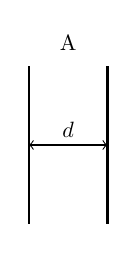
\begin{tikzpicture}
      \foreach \x in {0,1} \draw[thick] (\x,0)--+(0,2);
      \draw[<->] (0,1)--(1,1) node[midway,above]{$d$};
      \node at (.5,2.3){A};
    \end{tikzpicture}
    \hspace{.5in}
    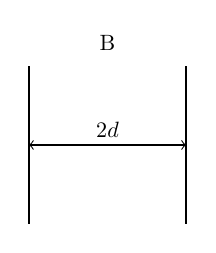
\begin{tikzpicture}
      \foreach \x in {0,2} \draw[thick] (\x,0)--+(0,2);
      \draw[<->] (0,1)--(2,1) node[midway,above]{$2d$};
      \node at (1,2.3){B};
    \end{tikzpicture}
    \hspace{.5in}
    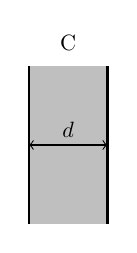
\begin{tikzpicture}
      \fill[lightgray] rectangle (1,2);
      \foreach \x in {0,1} \draw[thick] (\x,0)--+(0,2);
      \draw[<->] (0,1)--(1,1) node[midway,above]{$d$};
      \node at (.5,2.3){C};
    \end{tikzpicture}
    \hspace{.5in}
    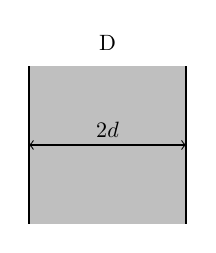
\begin{tikzpicture}
      \fill[lightgray] rectangle (2,2);
      \foreach \x in {0,2} \draw[thick] (\x,0)--+(0,2);
      \draw[<->] (0,1)--(2,1) node[midway,above]{$2d$};
      \node at (1,2.3){D};
    \end{tikzpicture}
  }
  
  \question Four parallel plate capacitors all have the same plate area and
  have the plate separations shown above. Both capacitors A and B have air
  between the plates, while the space between the plates of both capacitors C
  and D is filled with a dielectric slab of dielectric constant $\kappa=2$.
  Which of the following correctly ranks the capacitors in order of their
  capacitance from largest to smallest?
  \begin{choices}
    \choice $B>(A=D)>C$
    \choice $(A=C)>(B=D)$
    \choice $C>(A=D)>C$
    \choice $(B=D)>(A=C)$
    \choice $D>C>B>A$
  \end{choices}
\end{questions}
\end{document}
